\section{CLIP}\footnote{\url{https://en.wikipedia.org/wiki/CLIP}}

\subsection{CLIP-Seq}
\underline{c}ross-\underline{l}inking \& \underline{i}mmunoprecipitation \underline{p}rotocol (cross-linking immunoprecipitation-high-throughput sequencing)\footnote{\url{https://de.wikipedia.org/wiki/CLIP-Seq}}
\begin{itemize}
	\item Ultravioletes Licht für Cross-Linking
	\item UV-Licht cross linked NUR RNA mit Proteinen
	\item Induziert UV Mutation der RNA
	\item CIMS: \underline{C}ross-\underline{l}inking \underline{i}nduced \underline{m}utation \underline{s}ite
\end{itemize}

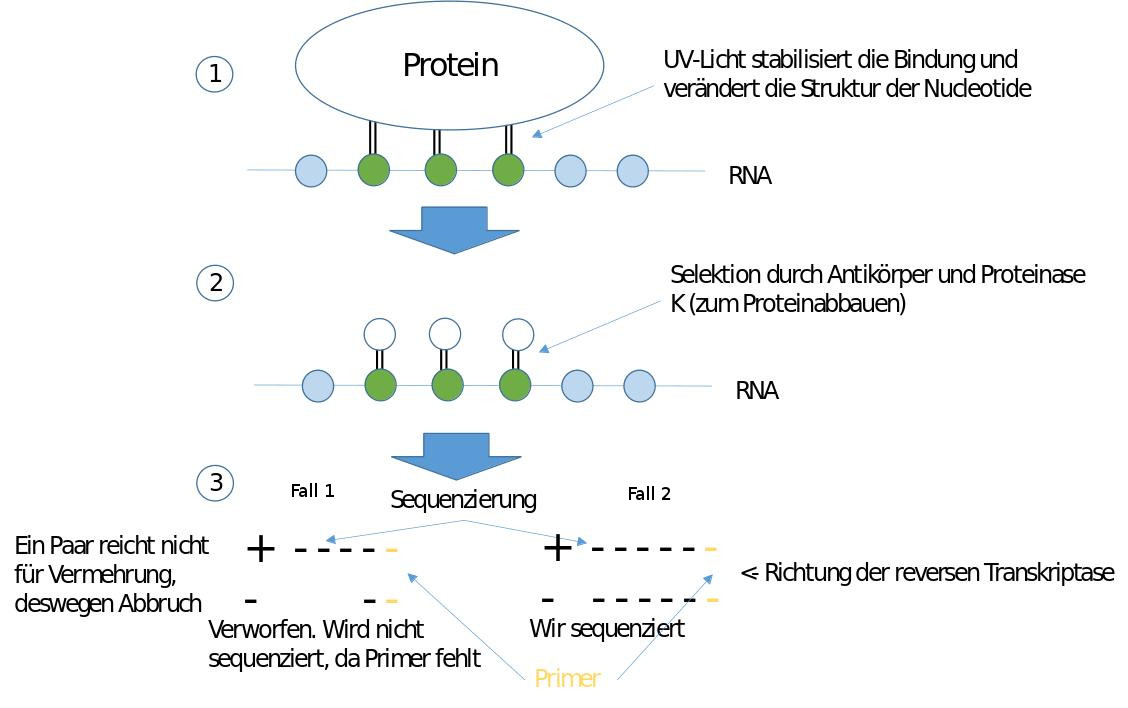
\includegraphics[width=1\textwidth]{lectures/160429/pix/clip_seq.jpg}
\\\\
Template ist per Definition Plus-Strang und dass durch die PCR erzeugte der Minus-Strang (auch wenn es in der Zelle anders ist).
\\\\
 - Fall Links und Rechts treten gleichzeitig auf\\
 - wird in vitro gemacht
\newpage
Mutation ist Bindungsstelle:
\begin{center}
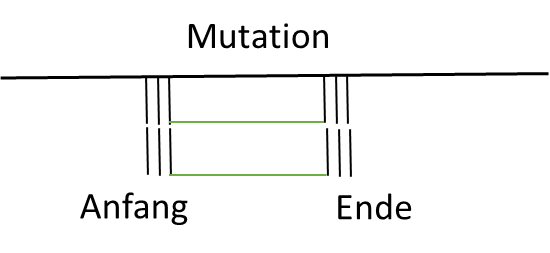
\includegraphics[width=0.5\textwidth]{lectures/160429/pix/mutation.png}
\end{center}

 - nach Häufungen schauen\\
 - hohe Sequenziertiefe benötigt

\subsection{ICLIP}
\underline{i}ndividual nucleotide–resolution \underline{c}ross-\underline{l}inking and \underline{i}mmunoprecipitation \underline{p}rotocol\footnote{\url{https://de.wikipedia.org/wiki/ICLIP}}
\\\\
- Schritt 1 und 2 wie bei CLIP-Seq\\
- Im Schritt 3 werden jetzt aber zirkuläre RNA erzeugt
\\\\
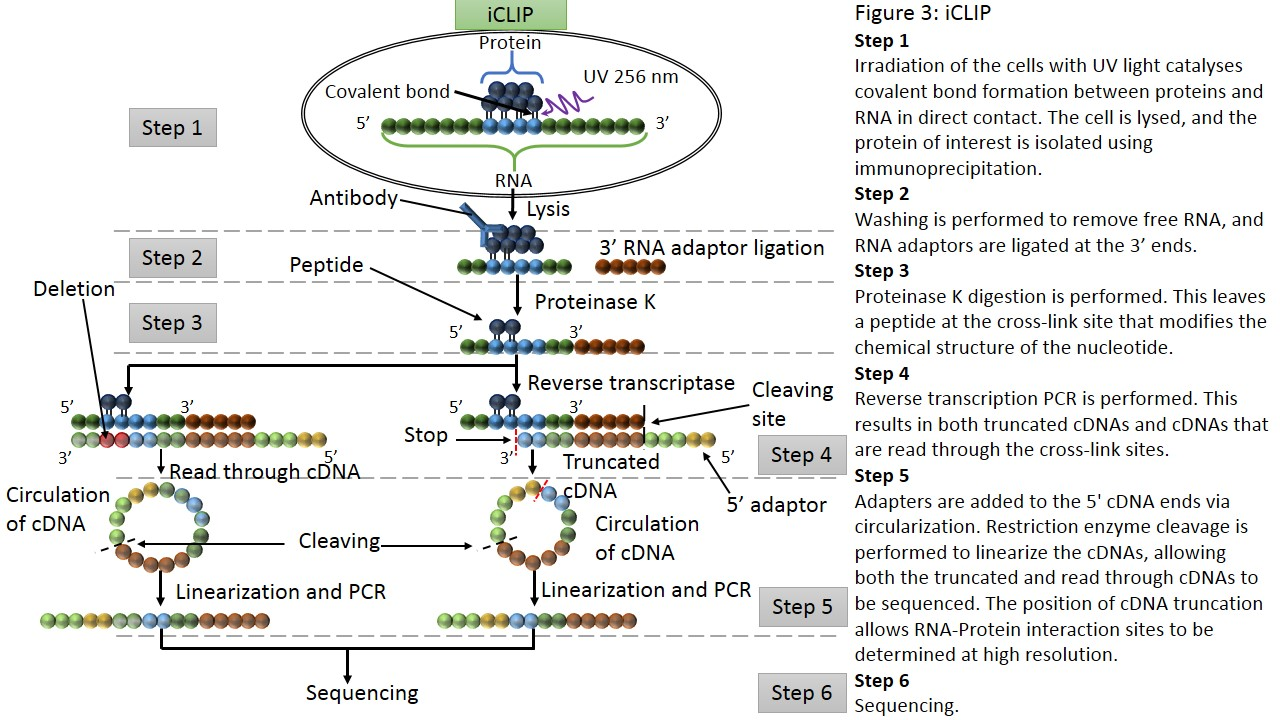
\includegraphics[width=1.2\textwidth]{lectures/160429/pix/iclip.png}

 - \textbf{Vorteil:} Beide Ergebnisse aus Schritt 5 können in Schritt 6 genutzt werden
\newpage
\subsection{PAR-CLIP}
\underline{P}hoto\underline{a}ctivable \underline{R}ibonucleoside-enhanced CLIP\footnote{\url{https://de.wikipedia.org/wiki/PAR-CLIP}}

\begin{itemize}
	\item Photoaktive (reagieren auf UV-Licht) Ribonucleoside -> Diese lassen wir in DNA einbauen
	\item UV-Licht für Cross Linking
	\item Cytosin ist photoaktiv, wird durch UV-Licht zu Uracil (welches in DNA zu Thymin wird)
	\item Antikörper um RNA Fragmente auszuwählen
\end{itemize}

\begin{tabular}{cc}
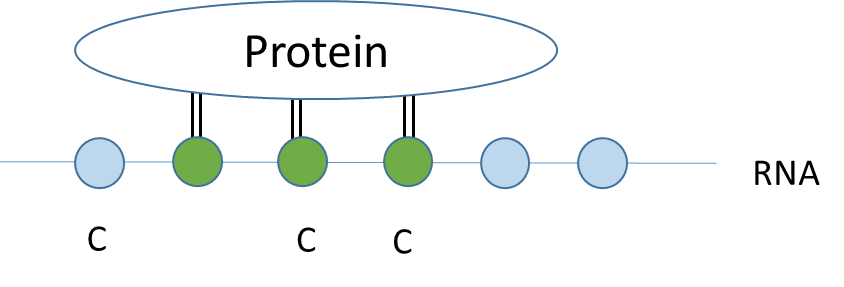
\includegraphics[width=0.5\textwidth]{lectures/160429/pix/par_clip1.png} & 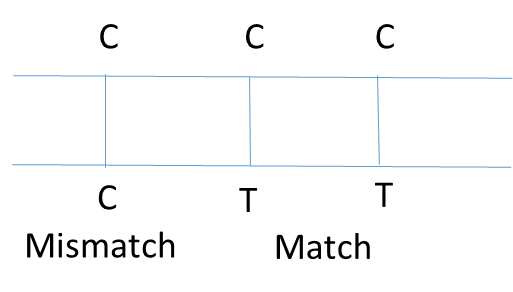
\includegraphics[width=0.5\textwidth]{lectures/160429/pix/par_clip2.png}
\end{tabular}

\textbf{\underline{Seeding:}} Transkription C$\rightarrow$T, Reads C$\rightarrow$T\\\\
\textbf{\underline{Alignment:}} angepasste Kostenfunktion(C$\rightarrow$T wird nicht bestraft). Dadurch nicht symetrische Kostenfunktion

\newpage

\section{Protein-Protein-Interaktion}\footnote{\url{https://de.wikipedia.org/wiki/Protein-Protein-Interaktion}}

Yeast Two-Hybrid System\footnote{\url{https://de.wikipedia.org/wiki/Hefe-Zwei-Hybrid-System}}:\\
 - benötigt: Wirtsorganismus: Hefe\\
 - erzeugt: Zwei Hybridproteine
\\\\ 
\textbf{\underline{Fragestellung:}} Interagiert Protein X (Coding DNA X) mit Protein Y (Coding DNA Y)?

Normalfall:\\
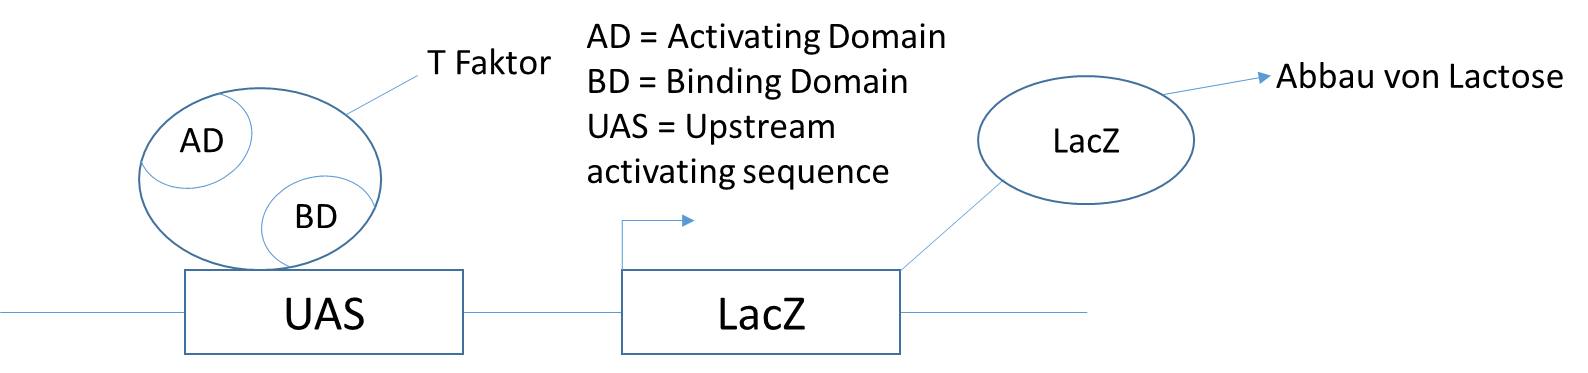
\includegraphics[width=1\textwidth]{lectures/160429/pix/ppi1.png}
\begin{itemize}
	\item Coding DNA X und Binding Domain von GAL4 werden in Vektor (=Stück zirkuläre DNA in die ich Proteine binden kann) kloniert
	\item Vektor mit coding DNA Y \& Activating Domain
	\item Beide Vektoren (haben auch Promotor) werden in Hefezelle eingeschleust
\end{itemize}

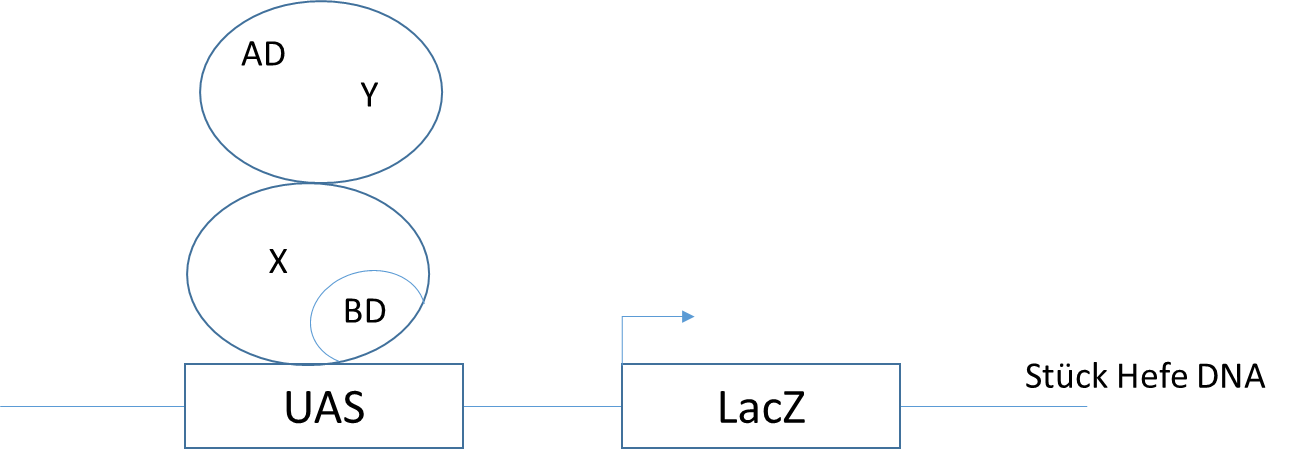
\includegraphics[width=1\textwidth]{lectures/160429/pix/ppi2.png}

\textbf{Welche Interaktionspartner hat Protein X?}
\begin{itemize}
	\item Erstellen einer Library (Vektor mit X und Vektor mit einem anderen Protein)
	\item Da wo Hefe auf Lactose wächst reagieren die Proteine
\end{itemize}

\textbf{Problem:}
\begin{itemize}
	\item X\&Y falten nicht in natürlicher Struktur und dies führt dazu dass sie nicht mehr binden können (false negativ)
	\item Das BD oder AD nicht gefaltet werden wie für ihre Funktion notwendig (false negativ)
	\item Vektor Klonierung funktioniert nicht immer (false negativ)
	\item Zufällige Aktvierung von Lac Z (false positiv von 80\%) $\rightarrow$ man bekommt nur die Info ob Hefe wächst, aber nicht wie stark
\end{itemize}

In Hefe kennt man ca-50\% aller Interaktionen (Interaktom). Mensch: 30\% des Interaktom bekannt.